\section{Auswertung}

\subsection{Charakteristik des Geiger-Müllerzählrohrs}

Die gemessenen Daten zur Charakteristik des Geiger-Müllerzählrohrs sind in der Tabelle \ref{tab:ogemessdaten}
angegeben. Dabei ist die Zählrate gemäß der Poisson-Statistik verteilt, somit lässt sich der Fehler auf die Zählrate gemäß $\sqrt{N}$
bestimmen.

Zunächst sollen die Messpunkte mit einem Fehlerbalken in ein Diagramm eingezeichnet werden und anschließend soll entlang des Plateau-Bereiches
eine lineare Ausgleichsgerade erstellt werden.

\begin{figure}[h]
  \centering
  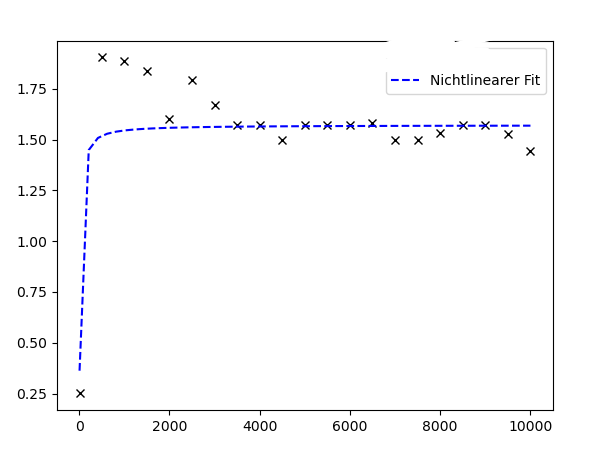
\includegraphics[width=\textwidth]{build/plot1.pdf}
  \caption{Messdaten und Fehlerbalken der Geiger-Müller Charakteristik}
  \label{fig:plot1}
\end{figure}